%
% This is the LaTeX source for the notes of Lecture 1; please use this as a
% template file for your scribe notes, and follow its style as far as possible.
%

\documentclass[twoside]{article}
\usepackage[colorinlistoftodos]{todonotes}
\usepackage[english]{babel}
\usepackage[hidelinks]{hyperref}
\usepackage[utf8]{inputenc}
\usepackage{amsfonts}
\usepackage{amsmath}
\usepackage{amssymb}
\usepackage{breqn}
\usepackage{caption}
\usepackage{graphicx}
\usepackage{lipsum}
\usepackage{mathtools}
\usepackage{multicol}
\usepackage{soul}
\usepackage{subcaption}
\usepackage{tikz}
\usepackage{xcolor}

\graphicspath{ {images/} }

\setlength{\oddsidemargin}{0.25 in}
\setlength{\evensidemargin}{-0.25 in}
\setlength{\topmargin}{-0.6 in}
\setlength{\textwidth}{6.5 in}
\setlength{\textheight}{8.5 in}
\setlength{\headsep}{0.75 in}
\setlength{\parskip}{0.1 in}


% Setup Blue URLS
\newcommand{\myul}[2][black]{\setulcolor{#1}\ul{#2}\setulcolor{black}}

% Paragraph indents in latex are on by default.  This next blurb changes indents to "specified only"
% You can use \indent to indent
\newlength\tindent
\setlength{\tindent}{\parindent}
\setlength{\parindent}{0pt}
\renewcommand{\indent}{\hspace*{\tindent}}

%
% The following commands set up the lecnum (lecture number)
% counter and make various numbering schemes work relative
% to the lecture number.
%
\newcounter{lecnum}
\renewcommand{\thepage}{\thelecnum-\arabic{page}}
\renewcommand{\thesection}{\thelecnum.\arabic{section}}
\renewcommand{\theequation}{\thelecnum.\arabic{equation}}
\renewcommand{\thefigure}{\thelecnum.\arabic{figure}}
\renewcommand{\thetable}{\thelecnum.\arabic{table}}


%
% Convention for citations is authors' initials followed by the year.
% For example, to cite a paper by Leighton and Maggs you would type
% \cite{LM89}, and to cite a paper by Strassen you would type \cite{S69}.
% (To avoid bibliography problems, we redefine the \cite command.)
% Also commands that create a suitable format for the reference list.
\renewcommand{\cite}[1]{[#1]}
\def\beginrefs{\begin{list}%
		{[\arabic{equation}]}{\usecounter{equation}
			\setlength{\leftmargin}{2.0truecm}\setlength{\labelsep}{0.4truecm}%
			\setlength{\labelwidth}{1.6truecm}}}
	\def\endrefs{\end{list}}
\def\bibentry#1{\item[\hbox{[#1]}]}

% Use these for theorems, lemmas, proofs, etc.
\newtheorem{theorem}{Theorem}[lecnum]
\newtheorem{lemma}[theorem]{Lemma}
\newtheorem{proposition}[theorem]{Proposition}
\newtheorem{claim}[theorem]{Claim}
\newtheorem{corollary}[theorem]{Corollary}
\newtheorem{definition}[theorem]{Definition}
\newenvironment{proof}{{\bf Proof:}}{\hfill\rule{2mm}{2mm}}

% **** IF YOU WANT TO DEFINE ADDITIONAL MACROS FOR YOURSELF, PUT THEM HERE:
\DeclareMathOperator{\sgn}{sgn}
\DeclareMathOperator{\contrib}{contrib}
\newcommand{\pp}{\mathcal{P}}
\newcommand{\ee}{\mathcal{E}}

\begin{document}
	%FILL IN THE RIGHT INFO.
	%\lecture{**LECTURE-NUMBER**}{**DATE**}{**LECTURER**}{**SCRIBE**}
	

	\section{Introduction}
	This project presents an original algorithm for automated harmony generation: given a sequence of $n$ melodies, the algorithm uses iterative random walk via Markov Chains with simulated annealing (Metropolis-Hastings) to generate a sequence of $n$ accompanying chords intended over time to approach a maximum score, as computed by an objective fitness function. For this type of problem, it is not possible to establish from the outset what the single most probable (highest-scoring) sequence of chords is going to be for a given melodic input; this is true even if we were to somehow assume a universally fixed set of rules that apply to music as a whole (of course, such fixed rules do not exist even within the context of a single style of music, whether it be baroque, impressionism, contemporary popular music, or otherwise). In the interest of experimentation, I have devised separate scoring functions for three distinct musical "styles" (See Subs. 1.4.5 for more details), effectively creating three different types of chord sequence distributions, and using the above-stated optimization approach to try to sample from the highest-scoring portion of the solution distribution space for each style. This project is inspired by, and is an attempt to expand upon, a number of related works to be discussed in Sec. 1.3, which utilize various methods ranging from genetic algorithm to MDP (Markov Decision Processes). The codebase and test cases for the project can be accessed at: \href{https://github.gatech.edu/ypark346/MCMC}{\color{blue} \myul[blue] {https://github.gatech.edu/ypark346/MCMC}}.
	\\\\
	Sec. 1.2 provides a brief primer on notes, chords and harmony as an introduction to the reader to understanding some of the musical syntax underlying my proposed algorithm. Sec. 1.3 outlines some of the related work on this subject, followed in Sec. 1.4 by a description of the algorithm. We finish in Secs. 1.5 and 1.6 with a discussion and analysis of the results and ideas for future improvement.
	\section{Musical Background}
	In music, a note pertains to a sound with a given frequency (pitch), amplitude (loudness) and duration (temporal interval, i.e. how long the sound lasts). In western classical music dealing with discrete pitches, there are a total of twelve distinct "pitch classes": C, C\#, D, D\#, E, F, F\#, G, G\#, A, A\#, B. Two notes belong to the same "pitch class" and are thus considered equivalent if their frequency ratios can be expressed in terms of a power of two (e.g. $2:1$, $4:1$, etc.). For instance, when a note located 12 semitones above another, the interval is called an octave (where the upper note has twice the frequency of the lower note), and thus both notes belong to the same pitch class. Here, a semitone refers to the frequency interval between two adjacent notes in a 12-tone equal temperament scale, which is a scale commonly used in Western music with each adjacent pair of pitches separated by an equal frequency interval ratio of precisely $\sqrt[12]{2}$ (notice that raising this quantity to the power of 12 results in an octave, with a frequency ratio of 2:1 as previously stated). While different types of scales  exist, for purposes of this project we are only concerned with discrete notes in the 12-tone equal temperament scale, similar to the notes played on a modern piano or a keyboard.
	\\\\
	A melody is defined as a group of individual notes played in some sequential order and rhythm, and is widely considered to be the central part of a musical piece. Harmony is also a group of notes, except that they typically consist of a sequence of chords played below the melody. A chord, in turn, is defined as a set of two or more notes played simultaneously, and is traditionally comprised of combinations of two to four distinct notes each (respectively termed dyad, triad and tetrad). Most related work on this subject (discussed in the next section) is concerned with tetrads at most, and is sometimes limited to triads or simpler chords.
	\\\\
	The purpose of harmony is to accompany the melody such that the result has aesthetic merit, the evaluation of which depends on many factors -- some of which may be arbitrary, though many are based on well-established rules of music theory, at least in the Western classical tradition. Among these rules, two are of particular interest for purposes of the current project: 1) tonality and 2) chord progression. 
	\begin{enumerate}
		\item[1.]
		Tonality, in a broad sense, refers to the arrangement of notes and/or chords in a way that is centered around the tonic note (i.e. the first note of a scale in a given key signature, such as the note C in a C-major scale, or the note G\# in a G\#-minor scale) of a given musical piece, and that tends towards harmonic stability with respect to that tonic. A harmony is generally considered "stable" if the frequency ratios of every pair of notes making up all or most of the chords in a sequence can be expressed in terms of small integers (usually $< 10$) within the framework of a just scale (meaning such chords are "consonant"), and the remaining "dissonant" chords tend to transition or resolve to consonant chords. As an illustration, among the most common and stable chords is the major (and minor) triad, consisting of three notes: tonic, major (or minor) third, and perfect fifth. Taking the C major triad with the notes C, E, G in ascending order as an example, the pair (C, E) is separated by 4 semitones and has a frequency ratio of $5:4$; (E, G) is separated by 3 semitones and has a ratio of $6 : 5$; and (C, G) is separated by 7 semitones and has a ratio of $3 : 2$. By contrast, a dissonant chord such as a tritone has a frequency ratio of $64:45$.
		\\\\
		(Here, the observant reader may have noticed that, within the equal temperament scale (with each semitone being exactly $\sqrt[12]{2}$ in frequency interval ratio), the aforementioned ratios for each pair are slightly off: (C, E) for example has a ratio of $\left(\sqrt[12]{2}\right)^4 \approx 1.2599 \neq 5:4 = 1.25$. However in a just scale framework (otherwise known as "harmonic tuning"), the ratios are exactly correct as stated. The reason for this difference between just scale and equal temperament scale has a long history, but for present purposes it suffices to say that the latter is an approximation of the intervals of just scale, with the chief benefit being that due to the constant ratio between every semitonic interval, it is easy to transpose a piece of music to any key signature without the resulting piece sounding "out of tune". Due to this fact, the equal temperament scale has been widely adopted in Western music beginning in the 18th century.)
		\\\\
		Aside from stable chords, the tonality of a musical piece also depends on the relation and directionality of chord progressions, as discussed below.
		\item[2.]
		Chord progression is a sequence of chords that, at least in tonal music, have the function of reinforcing (or sometimes contradicting for effect) the tonic of a given key signature. Often expressed in Roman numerals, chord progressions are the bedrock of traditional and popular Western music. For instance, blues musicians often utilize variations of the I-IV-I-V-IV-I chord progression in their compositions. In the C major key, the preceding progression can be expressed in terms of major triads involving the following sequence of tonic notes: C-F-C-G-F-C. A particularly important subset of chord progressions is the cadence, which is a sequence of two or more chords used to conclude a musical phrase or section. Two of the most common cadences are "perfect" and "plagal", respectively notated V-I and IV-I. The above-referenced blues chord progression contains examples of the latter.
	\end{enumerate}
	Finally, a quick word on interval notation and inversion, which are also germane to the current project and will be referenced again in later sections. Not to be confused with frequency intervals, interval notation is a way to represent chords without information on the specific keys comprising them. This loss of information regarding the keys is compensated by the fact that interval notations are useful when considering the "weight" or "likelihood" of a particular type of chord or of a particular type of chord-to-chord transition. For instance, a chord composed of the notes C-E-G (the C major triad) and another composed of Eb-G-Bb (Eb major triad) can be represented by the same interval notation [4, 7], indicating that the second note of the chord is 4 semitones above the first, and the third note is 7 semitones above the first. Inversion is the process of "sliding" a given chord in a way that cycles through the various ways of ordering the notes comprising the chord; to demonstrate, given the triad C-E-G, the first inversion is E-G-C and the second is G-C-E, with respective interval notations of [3, 8] and [5, 9]. Inversions provide additional variety to a chord representation without changing its core nature, which in the above example is the C-major triad.
	\\\\
	It should also be noted that for purposes of the project, every element within an interval notation consists of integers between 1 and 11 inclusive sorted in ascending order, and any chord that would contain an element $e_c$ exceeding this value (e.g. contains a pair of notes separated by a semitonic interval of 12 or greater, i.e. an octave or more) is instead decremented by performing the following modulo operation: $e_c = e_c \mod 12$. This is based on the concept mentioned earlier that a note is in the same pitch class as another that is 12 semitones (or any multiple thereof) below or above it. As an illustration, triads C-E-G and C-G-E, respectively arranged from lowest to highest in that order, are considered equivalent for purposes of the algorithm and have the same interval notation [4, 7] (the latter triad would have an interval notation of [7, 16] had it not been for the above-referenced modulo operation and the subsequent sort in ascending order); hence, they are not inversions of each other.

	\section{Summary of Related Work}
	In an earlier research by Horner \& Ayers, "Harmonization of Musical Progressions with Genetic Algorithms" (1995), a genetic algorithm was employed to tackle the task of voice leading, which is the process of creating chord progressions (historically in 4-part chorale music) in a way that each of the individual parts (bass, tenor, alto, and soprano) in isolation transitions in a "smooth" manner. However, their work was on a more constrained version of the current problem, since all of the initial chord sequences (and not just the melodic sequence) were provided as input, and the task consisted of mutating the given chords (e.g. by inverting them) to improve the overall voice leading.
	\\\\
	In "Harmonizing Chorales by Probabilistic Inference" (2005), Allan \& Williams used Hidden Markov Models (HMM) to generate harmonies given the input of a melodic sequence. Chorale works by composer J.S. Bach were used for training data, and first-order Markov assumptions were made regarding the transition probabilities of the chord sequences ("hidden" states), where the conditional probability of $c_t = $ chord at time $t$ depends only on the previous chord $c_{t-1}$:
	$$P(c_t | c_{t-1}, ..., c_0) = P(c_t | c_{t-1})$$
	Similar assumption was made regarding the conditional probability of the observed event, i.e. a melodic note $y_t$, which depends only on the current chord:
	$$P(y_t | c_t, ..., c_0, y_{t-1}, ..., y_0) = P(y_t | c_t)$$
	In their work, the "hidden" chord states were actually visible during training, so that emission and transition probabilities could be learned directly from the training data set. The Viterbi algorithm (Forney, '73) was then used to find the most probable sequence of states (i.e. chord sequence) given the input melody. However, the harmonization was limited to one musical style only (Bach) due to the nature of the training data; another limitation was that the algorithm only considers chords in terms of their interval notations and has no conception of key signatures.
	\\\\
	Yi \& Goldsmith, in "Automatic Generation of Four-Part Harmony" (2007), used MDP (Markov Decision Process) for generating chord progressions accompanying an input melodic sequence. In their model, a state is represented as a set of 10 variables $(S_1, A_1, T_1, B_1, S_2, A_2, T_2, B_2, S_3, P)$, where $S_i$, $A_i$, $T_i$ and $B_i$ respectively refer to the soprano (i.e. melody), alto, tenor and bass pitch in index $i$, with $i$ denoting the relative positions of the chords in an adjacent two-chord sequence as well as the the following melody (indicated by $S_3$), and $P$ refers to the position of the first chord in the current state. In other words, a state consists of the previous chord, current chord, and the next melody. Two specific rules are taken into account in computing the utility a.k.a. score of a state: 
	\begin{enumerate}
		\item[1.]
		preference is given to a chord in which one or more notes therein belong to the same pitch class as the corresponding melody; and 
		\item[2.]
		preference is given to a chord-to-chord transition that is in the form of either a perfect or a plagal cadence. 
	\end{enumerate}
	From a given state, then, the next state is computed by picking the best action from a set of 7 possible actions (with an action pertaining to a particular type of triad to be assigned to the chord accompanying $S_3$): tonic, supertonic, mediant, subdominant, dominant, submediant, or leading tone (respectively labeled I, ii, iii, IV, V, vi, or vii). Once a chord is chosen, it is randomly inverted before being assigned to accompany $S_3$. The new state is $(S_1', A_1', T_1', B_1', S_2', A_2', T_2', B_2', S_3', P')$, where $S_1' = S_2,A_1'=A_2,T_1'=T_2,B_1'=B_2, P'=P+1$, and $A_2',T_2',B_2'$ comprise the newly generated chord to accompany $S_2'=S_3$. 
	\\\\
	In computing the "best" action at each state, a modified SPUDD algorithm (Hoey, et. al. "SPUDD: Stochastic Planning using Decision Diagrams" (1999)) is used, with an iterative approximation algorithm ($n$-stage-to-go value functions $V^n$)to approach an optimal policy for the next state $s$:
	$$V^n(s)=R(s)+\max_a[\gamma \sum_{s' \in S}Pr(s'|s,a)V^{n-1}(s')]$$
	where $V^n(s)$ pertaining to a state $s$ gives the maximum utility score for that state in terms of all possible previous states $s'$, $R(s)$ is the immediate reward score for state $s$ in a vacuum, $Pr(s'|s,a)$ is the conditional probability that $s'$ was the previous state given that an action $a$ was chosen during the previous state and that the current state is $s$, and $0 \leq \gamma < 1$ is a preset discount rate. 
	\\\\
	While the algorithm generated tonal harmonies that made musical sense, the tight constraints on the number of actions (limited to 7 triads, and no tetrads supported) along with the above-referenced two simple rules meant that the generated harmonies focused almost entirely on tonality at the expense of variety and complexity.
	\section{Description of the MCMC-MH Harmonizer}
	I now proceed to describe the core algorithm employed in the current project. The state space $\Omega$ consists of a set of all "valid" chord sequences, where a chord sequence is defined as $C = \{c_1,...,c_n\}$. Each chord consists of 4 parts: $\forall i, 1 \leq i \leq n, c_i=\{p_1, ..., p_4\}$, where $p_1$ thru $p_4$ respectively denote the bass, tenor, alto and melody parts, and $v(p_j) =$ an integer pitch value assigned to part $p_j$. We assume that $\forall j \in \{1,2,3,4\}, 0 \leq v(p_j) \leq Q = 87$ (modeled after modern piano / keyboard, which consists of 88 pitches total). Of these, the melody is given as part of the input and, thus $\forall i, p_4 \in c_i$ is fixed and unchanging. For convenience, we can separately notate  the input melodic sequence as $M=\{m_1,...,m_n\}$, where $m_i = p_4 \in c_i$.
	\subsection{Validity Constraints}
	For purposes of this project, a chord sequence $C$ is deemed "valid" IFF, for each $c_i \in C$, all of the following constraints are met:
	\begin{enumerate}
		\item[(1)]
		$w_e(c_i) \neq -\infty$, where $w_e=$ a weight value assigned to $c_i$.
		\item[(2)]
		$w_t(c_i, c_{i-1}) \neq -\infty$, where $w_t=$ a weight value assigned to the chord progression from $c_{i-1}$ to $c_i$.
		\item[(3)]
		$\forall j \in \{1,...,4\}$, $v(p_j) \leq v(p_{j+1})$.
		\item[(4)]
		For each $c_i, m_{i-1}$ and $m_{i+1}$, and $\forall j \in \{1, 2, 3\}$, 
		\begin{enumerate}
			\item[i)]
			$v(p_j) \in c_i \leq v(m_{i+1})$, and
			\item[ii)]
			$v(p_j) \in c_i \leq v(m_{i-1})$.
		\end{enumerate} 
	\end{enumerate} 
	where $w_e, w_t$ in (1) and (2) are pre-set weights using domain knowledge based on classical Western music theory indicating the fact that certain types of chords, and certain types of chord-to-chord progressions, are more common/acceptable than others, while other types which are virtually unheard of are given values of $-\infty$; (3) indicates that the parts in a chord should be in nondecreasing order (e.g. the bass cannot be above the alto); and (4) is based on one of the guidelines pertaining to voice leading that the bass, tenor, and alto notes should at all times stay at or below not just the current but also adjacent melodies. There are many other rules that could be implemented as additional constraints, but for the sake of simplicity we limit them to the ones stated above. As part of the initialization step, and to help facilitate transitions between states, all unisons and dyads are assigned weight values of $w_e \neq -\infty$.
	\\\\
	It should also be noted that the weights $w_e(c_i)$ and $w_t(c_i, c_{i-1})$ are assigned using the interval notations of the chords as parameters (see Sec. 1.2 for reminder on interval notation), and thus key signatures are irrelevant for this purpose. With few exceptions, inversions of $c_i$ are assigned the same weight as that for $c_i$; same goes for transitions between inversions of $c_i$ and $c_{i-1}$.
	\subsection{Markov Chain and State Transition}
	The task is to generate a chord sequence $C$ given $M$ that approaches a maximum score computed using an fitness function (to be detailed in Sec. 1.4.4). To do this, we begin from an initial state $X_1 \in \Omega$ where for every $c_i \in X_1$, $v(p_1)=v(p_2)=v(p_3)=\min(v(m), \forall m \in M)$, and $v(p_4)=v(m_i)$. This initial state is guaranteed to be valid since each chord $c_i \in X_1$ is either a unison or a dyad (chords consisting respectively of one or two distinct pitch classes) that meet all four constraints outlined in Sec. 1.4.1 above (as a reminder, all unisons and dyads have weight values of $w_e \neq -\infty$). Transition between states is governed by the following scheme: from a state $X_t$ at time $t \geq 1$,
	\begin{enumerate}
		\item[(1)]
		Choose a chord $c_i \in X_t$ u.a.r.
		\item[(2)]
		Choose a part $p_j \in c_i$, $j \in \{1,2,3\}$ u.a.r.
		\item[(3)]
		Choose a new pitch value $v(p_j) \in \{0,...,Q\}$ for $p_j$ u.a.r.
		\item[(4)]
		Let $X'=$ the chord sequence with the above change.
		\item[(5)]
		If $X'$ is "valid":
		\begin{itemize}
			\item 
			Compute the score $s'$ for $X'$. 
			\item 
			If $s' > s$ (where $s=$ score for $X_t$), then let $X_{t+1} = X'$. If not, let $X_{t+1} = X'$ with probability $e^{-(s - s')/T}$, and $X_{t+1} = X_t$ otherwise. Here, $T$ is a temperature value, which decays over time and is governed by the following formula: $T = c / \sqrt{t}$, where $c=$ a preset cooling rate.
		\end{itemize}
	\item[(6)]
	Otherwise, set $X_{t+1} = X_t$.
	\end{enumerate}
	As a hypothetical exercise, if we imagine for a moment that there had been no constraints regarding a chord's validity and no objective scoring function, then the above would be a simple case of an ergodic Markov Chain with a uniform stationary distribution $\pi$, since in that case, the chain would be strongly connected and aperiodic, and for every pair of adjacent states $X_t,Y_t \in \Omega$ (where $X_t$ and $Y_t$ have all but one pitch in common), $P(X_t,Y_t)$ would equal $P(Y_t,X_t)=\frac{1}{3n(Q+1)}$. And in this ideal scenario, the mixing time would be simple enough to derive using a path coupling scheme in which the same chord, part and pitch value $c_i, p_j, v(p_j)$ are chosen u.a.r. for both $X_t$ and $Y_t$. Then the probability of a "good outcome" where $X_{t+1}=Y_{t+1}$ would equal $Pr(X_{t+1}=Y_{t+1})=\frac{1}{3n}$. With this coupling scheme, there is no probability of a "bad outcome" where the no. of disagreeing pitches increases after a time step (which we'll notate as $Pr(|D_{t+1}|>|D_t|) = 0$), and hence the expected value for $|D_{t+1}|$ is $E[|D_{t+1}|]=|D_t| - \frac{1}{3n} = |D_t|(1 - \frac{1}{3n|D_t|}) \leq |D_t|(1 - \frac{1}{3n})$ (since $|D_t| \leq 1$), and via the path coupling lemma, $E[|D_{t+1}|] \leq |D_0|(1 - \frac{1}{3n})^t \leq 3n(1-\frac{1}{3n})^t \leq 3ne^{-t/3n} \leq 1/4$ for $t \geq n \ln (12n)$, meaning $T_{mix}=O(n \log n)$. (Note that it is also possible to reach the same conclusion by realizing that this task reduces to the coupon collector problem.)
	\\\\
	In actuality, however, validity constraints and scoring functions are necessary to ensure that a chord sequence abide by at least a minimal set of guidelines in classical music theory pertaining to voice leading, chord progressions and tonality, a fact that leads to uncertainty regarding the mixing time and is the reason for my employing the Metropolis-Hasting algorithm as given above.
	\subsection{Ergodicity}
	While one may raise the question of whether the Markov Chain with the above constraints is even ergodic, we can show ergodicity as follows. First, it is clear that the chain is aperiodic, since $P(X, X) > 0$ for all $X \in \Omega$.	Next, we can establish irreducibility as long as we ensure that the weights $w_e$ and $w_t$ satisfy certain requirements. Recall Sec. 1.2 and the definition of pitch class, and let $\gamma(p)$ denote the specific pitch class that a single part (i.e. $p$) of a chord belongs to. Then, $\forall c,C$ where $c \in C, C \in \Omega$, the weights have been set to satisfy the following requirements:
	\begin{enumerate}
		\item [(1)]
		 $w_e(c) \neq -\infty$ if $\exists p, p' p'' \in c$ such that $\gamma(p) = \gamma(p') = \gamma(p'')$.
		\item [(2)]
		$\forall p, p' \in c$, if $\gamma(p) \neq \gamma(p')$ (and $c$ is a valid chord), then let $c' = $ a new chord consisting of 3 parts (one of which must be the melody part) in $c$ arranged in the same nondecreasing order, and $\forall c', w_e(c') \neq -\infty$.
		\item[(3)]
		$\forall c_{i-1},c_i \in C$, $w_t(c_i, c_{i-1}) \neq -\infty$.
	\end{enumerate}
	Informally, (1) simply states that $w_e > -\infty$ for all unisons and dyads. (2) states that given a valid tetrad (chord consisting of 4 notes that each belong to a distinct pitch class), any triad formed using the pitches from that tetrad is also valid. Finally, (3) states that all transitions between adjacent valid chords are given weights of $w_t > -\infty$ and are thus allowed.
	\\\\
	Assuming the above requirements are satisfied, it is possible to transition from any valid state (eventually) to any other valid state. To see how, we consider for the sake of simplicity a single chord $c_i$ within an arbitrary valid state, and can extrapolate the below scheme to all chords within that state:
	\begin{itemize}
		\item
		If $c_i$ is a unison, it is clear it can be mutated into any valid dyad, by selecting the bass note and moving it downward by the number of semitonic intervals needed. (Note that there is at most one possible valid unison for $c_i$: the unison containing the melody, and only if the previously stated requirements $v(p_j) \leq v(m_{i+1})$ and $v(p_j) \leq v(m_{i-1})$ would be satisfied; if not, there is no valid unison chord for that melody, and a dyad is the simplest valid chord.) Choosing the bass note and moving it downward to form a valid dyad ensures that the requirement $\forall j \in \{1,2,3,4\}, v(p_j) \leq v(p_{j+1})$ is satisfied (alternatively, we can choose any non-melodic note, move it downward, and then re-assign the parts so that they are sorted in nondecreasing order).
		\item
		If $c_i$ is a valid dyad, it can be mutated into any valid triad. Either both distinct pitch classes forming the dyad belong to that triad, or only one of them, the melody pitch class, does. (At least the melody must belong to the triad because every chord contains the melody.) If both pitch classes of the dyad belong to the triad, we can pick a note and move it to the necessary third position to form that triad, sorting and re-assigning the positions (bass, tenor, alto) as needed to satisfy the requirement that all parts be placed in nondecreasing order. If not, we can mutate the dyad into another dyad where the non-melody note is moved into a pitch class that belongs to the triad, and then proceed to move another note to the third position to complete the triad. Since every dyad is valid, it follows that every valid triad can be formed by mutating the right type of dyad.
		\item
		The mutation from a valid triad to a valid tetrad can follow the same logic as the dyad-triad mutation above. (Recall that as previously stated in one of the requirements, every valid tetrad can be formed from a valid triad, so we can mutate the triad as needed until all three pitch classes belong to the tetrad, then mutate the final note into the 4th position to form that tetrad.)
		\item
		Every valid chord consisting of $y$ distinct pitch classes, $2 \leq y \leq 4$, can be mutated into a valid chord consisting of $y-1$ distinct pitch classes, by simply picking a note and moving it to a duplicate position as another note (duplicate notes, as well as duplicate pitch classes, are equivalent and treated as if they were a single note for purposes of identifying the chord type -- hence for example, a chord where exactly two of its notes are duplicates is a triad). The only exception is that a dyad may not be mutated into a unison if doing so would violate the previously mentioned rule that $v(p_j) \leq v(m_{i+1})$ and $v(p_j) \leq v(m_{i-1})$.
	\end{itemize}
	Applying the above scheme to every chord, it is possible to get from any valid state to any other valid state; consequently, since the chain is strongly connected and aperiodic, it is ergodic, meaning there exists a unique stationary distribution.
	\subsection{Scoring Function}
	The fitness scoring function for a valid chord sequence, $C$, is defined as follows:
	$$\sum_{c_i \in C} \left(\beta(c_i) +  \alpha_{w_e} \cdot w_e(c_i) + \alpha_{w_t} \cdot w_t(c_i, c_{i-1}) + \delta(c_i, m_i, c_{i-1}) + \rho(c_i, k(m_i), \zeta(m_i))\right)$$
	where:
	\begin{itemize}
		\item
		$\beta(c_i) = $ pre-set baseline constant value assigned to the complexity level of chord $c_i$. It has four pre-set values depending on whether $c_i$ is a unison, dyad, triad or tetrad. As a default metric, triads and tetrads are given higher baseline values than unisons or dyads, although the values differ depending on musical styles (see Subs. 1.4.5).
		\item 
		$\alpha_{w_e}, \alpha_{w_t} = $ pre-set multiplier constants for emission weights and transition weights, respectively. Reflects the relative preference given to emission weights vs. transition weights in general.
		\item
		$\delta(c_i, m_i, c_{i-1}) = $ a non-positive value denoting a penalty in the event that the Hamming distance $H$ between $c_i$ and $c_{i-1}$, and/or the Hamming distance between $c_i$ and $m_i$, are greater than the pre-set, respective maximum distance constants $d_c$ and $d_m$, and is defined as follows:
		$$\delta(c_i, m_i, c_{i-1}) = d_{mult} \cdot [\min(0, d_c - H(c_i, c_{i-1})) + \min(0, d_m - H(c_i, m_i))]$$
		where $d_{mult}$ is a pre-set multiplicative constant.
		\item 
		$\rho(c_i, k(m_i), \zeta(m_i)) = $ a non-positive value denoting a penalty in the event that any of the notes comprising $c_i$ are incompatible with the perceived key signature (e.g. C, F, etc.) and scale (e.g. major / minor) for the melody $m_i$. (For example, if $m_i$ is associated with a C harmonic minor scale, consisting of the pitch classes C, D, Eb, F, G, Ab, B, and if $c_i$ is composed of the pitch classes $\{$G, Bb, Eb$\}$, then the pitch Bb is not contained in the given scale and thus $c_i$ is incompatible.) To explain further, the algorithm contains a greedy helper function that attempts to compute the most likely sequence of key signatures and scales for the given melodic sequence input (See Subs. 1.5.4 for more details). If any of the notes contained in $c_i$ do not belong to the computed key signature and scale pertaining to the melody $m_i$, then a penalty is assigned in accordance with a pre-set positive constant $k_{mult}$. Formally, let $k(m_i)$ indicate the computed key signature and $\zeta(m_i)$ indicate the computed scale for the melody $m_i$. Let $u(c_i, k(m_i), \zeta(m_i)) = $ true IFF all the notes in $c_i$ belong to the notes comprising the key signature $k(m_i)$ and the scale $\zeta(m_i)$. Then:
		$$\rho(c_i, k(m_i), \zeta(m_i)) = 
		\begin{cases}
		0, 			 & \text{if } u(c_i, k(m_i), \zeta(m_i)) = \text{true,}\\
		-k_{mult},& \text{otherwise.}
		\end{cases}$$
	\end{itemize}
	\subsection{Weights Pertaining to Different Musical Styles}
	In order to experiment with different musical styles in the automated harmonization, different values are assigned to the weights, multipliers, and/or other constants referenced in Subs. 1.4.4 depending on the selected style. Currently, there are 3 styles to choose from: classic/tonal, modern/atonal, and default (a combination of the former two styles). As an example, for the "classic/tonal" setting, triads are given much higher baseline values than tetrads, and very common triads (such as the major/minor triad) are given high $w_e$ values, and only the most common types of chord-to-chord transitions (such as perfect/plagal cadences) are given high $w_t$ values. By contrast, under the "modern/atonal" setting, tetrads are given the highest baseline scores, and a much broader set of chord types and chord transition types are given high weight values.
	\section{Results and Discussion}
	\subsection{Fitness Scores and Simulated Annealing}
	The efficiency of the algorithm and the quality of harmonization were tested for three different arbitrary values of $c=30,70,110$ (pre-set cooling rate, as defined in Subs. 1.4.2) and under the three different musical styles (as mentioned in Subs. 1.4.5). The graphs in Fig. 1.1 below display one example of the evolution of the fitness scores as the Markov Chain was run with $c=110$ for many iterations over one given melodic sequence, with one example graph shown for each of the 3 musical styles selected. We can see that due to Metropolis-Hastings and the simulated annealing process, the scores occasionally take a dip as worse states are explored, albeit with a smaller and smaller probability as the iterations continue. More complex musical styles (e.g. atonal) tend to have a higher upside as far as scores are concerned, since a greater number of chord and transition types are given higher weights.
	\begin{figure}[h]  % uses graphicx package. [h] forces figure to be placed "here", as opposed to default position like top of page
		\begin{center}  
			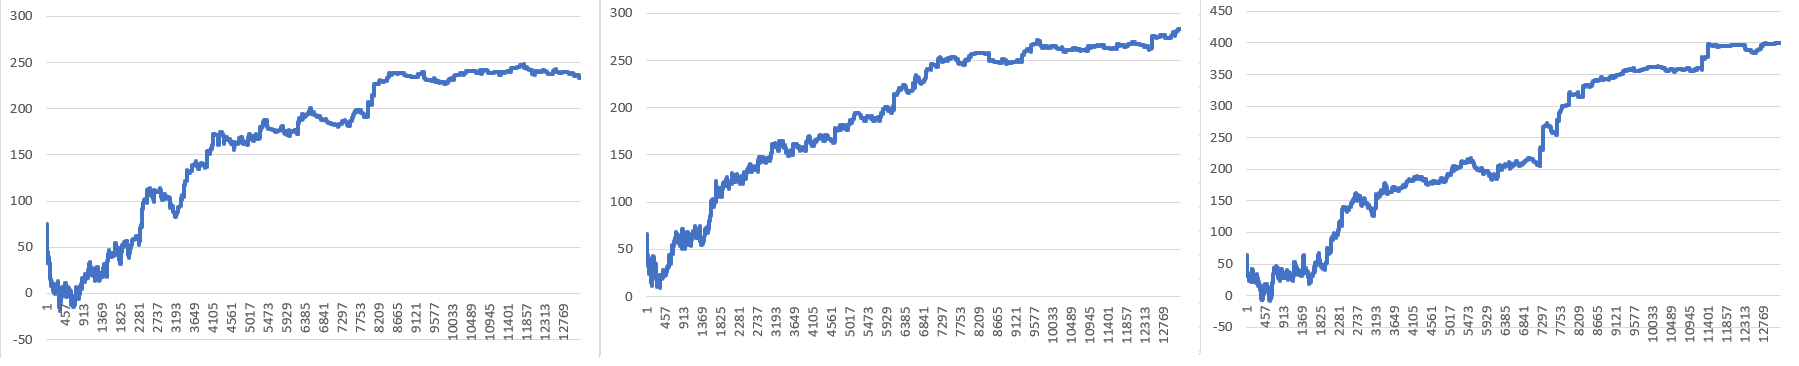
\includegraphics[scale=0.45]{Fig1.png}  
			\caption{\small \sl The fitness scores (vertical axis) as a function of the number of iterations (horizontal axis) of the Markov Chain. From left to right, the graphs pertain to the tonal, default, and atonal musical style.}
		\end{center}  
	\end{figure}
	\subsection{Mean, Median, and Standard Deviation}
	The table in Fig. 1.2 below shows the standard deviation, mean score, and median score over the course of one hundred trials each for every style and for each of the three $c$-values for the given melodic sequence. Somewhat surprisingly, the standard deviation for the atonal style with $c=70$ was the highest of all at 79.34, stemming from the fact that there was a larger number of outliers than there was under other settings. Despite these outliers, however, the overall mean and median scores were highest across all musical styles for $c=70$.
	\begin{figure}[h]  % uses graphicx package. [h] forces figure to be placed "here", as opposed to default position like top of page
		\begin{center}  
			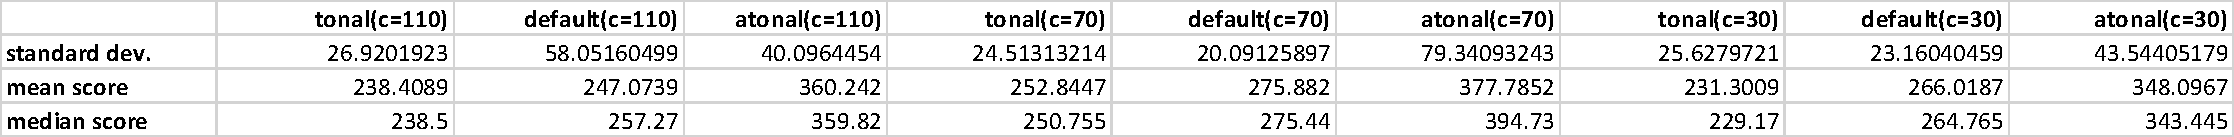
\includegraphics[scale=0.6]{Fig1_2.png}  
			\caption{\small \sl Stdev, mean and median scores for harmonizations pertaining to an example melodic sequence under various $c$-values and under different musical styles. 100 trials were run under the setting in each column.}
		\end{center}  
	\end{figure}
	\subsection{A Harmonization Example}
	An excerpt from actual harmonizations in the 3 styles for the melodic sequence is shown in Fig. 1.3 below. As can be seen, the differences in the musical nature of the chord outputs amongst the styles are significant. MIDI versions of the music can be accessed at the Github link referenced at the beginning of this paper.\footnote{The specific filenames pertaining to the scores are "test4 - frosty - tonal.mid", "test4 - frosty - default.mid", and "test4 - frosty - atonal.mid", in that order.}
	\begin{figure}[h]  % uses graphicx package. [h] forces figure to be placed "here", as opposed to default position like top of page
		\begin{center}  
			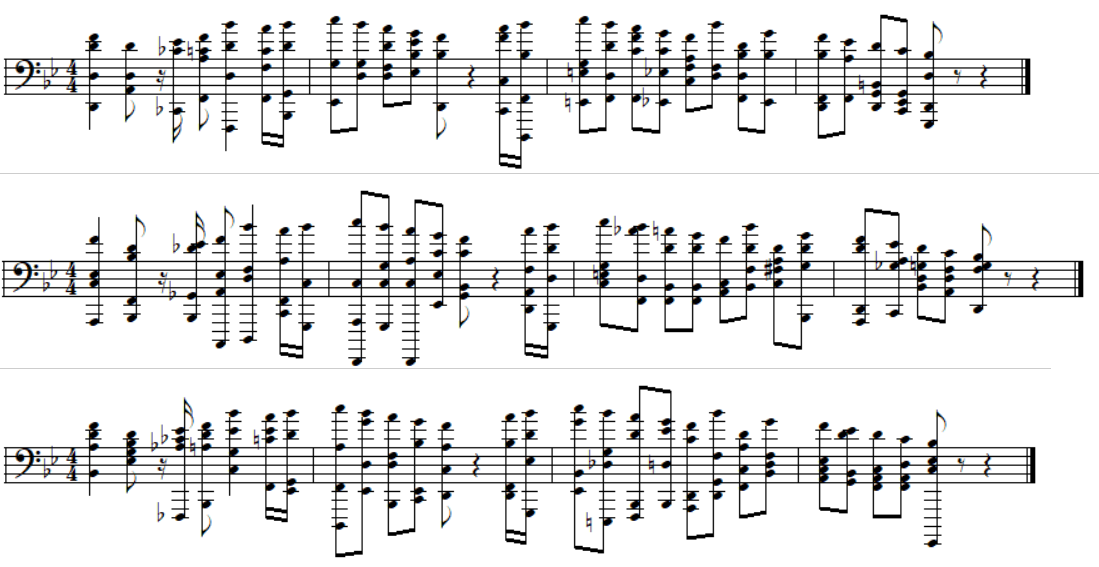
\includegraphics[scale=0.8]{Fig1_3.png}  
			\caption{\small \sl From top to bottom: generated harmonization for a melodic sequence in the tonal, default, and atonal style, with $c=70$. The melodic sequence is identical in all three cases.}
		\end{center}  
	\end{figure}
	\subsection{Known Issues}
	Two of the major inefficiencies the algorithm currently suffers from are (1) the presence of bottlenecks making certain state transitions difficult or time-consuming, and (2) imperfections in the key signature detection helper function (referenced in Subs. 1.4.4).
	\\\\
	To illustrate (1), transitions between complex chord types (e.g. tetrad-to-tetrad transitions), can be particularly troublesome due to the fact that many such transitions may need to undergo certain intermediate states perhaps comprised of simpler chord types, and one or more such intermediate states may either be invalid or result in lower interim fitness scores, meaning transitions to such intermediate states becomes less and less likely as the time steps are incremented. For example, consider the pair of tetrads shown in Fig. 1.4 (where we assume W.L.O.G. that the latter chord would result in a higher score than the current). It is clear that transitioning from the former to the latter tetrad would require a minimum of three time steps and two intermediate states (since the bass, tenor and alto notes all need to be changed). However, once we account for the fact that some tetrads are invalid or have lower weight values $w_e$ than the current chord, and that some of the possible paths between the first and second tetrad involve stepping through simpler chord types (triads, dyads and/or unisons) which tend to have lower baseline scores associated with them, it becomes intuitively obvious that transitions such as this one can represent bottlenecks in the chain. Sec. 1.6 outlines some ideas for dealing with this issue in a future work.
	\begin{figure}[h]  % uses graphicx package. [h] forces figure to be placed "here", as opposed to default position like top of page
		\begin{center}  
			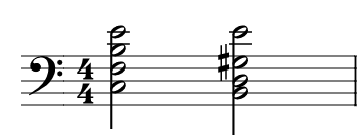
\includegraphics[scale=0.8]{Fig1_4.png}  
			\caption{\small \sl A pair of tetrads that require multiple intermediate states for transition.}
		\end{center}  
	\end{figure}
	\\\\
	Regarding (2), the current key signature and scale detection algorithm greedily assigns a single key signature and a scale to every melody in the given input so as to result in a sequence of assignments for the entire input, in such a way that minimizes both the total distinct number of key signatures/scales in the sequence, and the total number of changes in the same. This is based on the broad premise that key signatures rarely change within the context of a single musical piece. Still, the current algorithm tends to overfit the melody and result in more key/scale changes than is ideal, because it does not know how to differentiate between a melodic note that indicates a genuine change from the current key/scale and one that simply functions as a transient deviation therefrom (usually for musical effect); and the latter is far more common than the former. For instance, if all but one note in a given melodic sequence were to belong to a C major scale, the odd note will be registered by the algorithm as a key/scale change; however, it is quite probable that the note is a passing note, neighboring note, or a note otherwise serving a transient function. Hence, the chord generated for that odd melody will be weighted toward being compatible with a key/scale other than C major, even though a chord pertaining to C major may make the most musical sense.
	\section{Conclusion and Future Work}
	We have shown that it is possible to use the MCMC algorithm with simulated annealing to automatically generate a sequence of chords accompanying a given melodic input. Despite their shortcomings, the generated chord sequences are flexible enough to capture a variety of different musical styles and their respective aesthetic qualities represented as sets of heuristics.
	\\\\
	As part of future research, and to help alleviate the bottleneck problem identified in Subs. 1.5.4, it may be advisable to break down the harmonization task into two main subtasks: (1) Use MCMC to focus on generating the best quality of chords for the given input, ignoring the validity constraint having to do with voice leading (see Subs. 1.4.1 (4)) as well as the part of the scoring function pertaining to Hamming distances (see Subs. 1.4.4); and (2) Once the chords have been generated, use a second chain to focus on improving the voice leading and Hamming distances while making no changes to the chord types themselves, either via performing an inversion or raising/lowering one or more notes by an octave or more at each time step, and using simulated annealing and a separate scoring function for the state-to-state transition. The issues with the key/scale detection algorithm are a bit trickier to deal with, as the ability to differentiate between "genuine" and "transient" key/scale changes may require the algorithm to have a conception of overall musical intent, whether in terms of musical phrasing, extended ($n$-gram) transition sequences or otherwise. As a starting point, a subroutine may be devised that detects the most obvious cases of a melodic note serving a passing or neighboring function, guided by principles of classical music theory. Finally, to help further improve the scoring function, additional rules of music theory (e.g. parallel fifths, part overlap, parallel octave, etc.) could be imposed.
\end{document}